\documentclass[../main.tex]{subfiles}
\begin{document}
Un sottoprogramma in Java viene chiamato \underline{metodo}. I metodi vanno dichiarati fuori dal \code{main} e dentro alla classe.
Un sottoprogramma può essere una \underline{funzione} o una \underline{procedura}. Le funzioni ritornano qualcosa mentre le procedure no.

\begin{lstlisting}[style=java]
    private static int getUserInput(Scanner input, String message) {
        System.out.println(message);

        return input.nextInt();
    }
\end{lstlisting}
\textbf{Nota:} possono esistere due metodi con lo stesso nome purchè possiedano parametri diversi (overloading).

\vspace{1.5cm}
\subsection{Gestione della memoria}
\subsubsection{Tipi primitivi}
\begin{lstlisting}[style=java]
    int pippo = 15;

    //Questa funzione ritorna il doppio del valore passato come parametro
    makeItDouble(pippo); //Viene copiato il valore di pippo (value)
\end{lstlisting}
\begin{tikzpicture}[x=0.75pt,y=0.75pt,yscale=-1,xscale=1]
    %Shape: Rectangle [id:dp7998323845409867] 
    \draw   (154.67,50.33) -- (296.33,50.33) -- (296.33,217) -- (154.67,217) -- cycle ;
    %Shape: Rectangle [id:dp641168812213257] 
    \draw   (398,49.67) -- (539.67,49.67) -- (539.67,216.33) -- (398,216.33) -- cycle ;
    %Shape: Rectangle [id:dp10812800600084915] 
    \draw  [color={rgb, 255:red, 208; green, 2; blue, 27 }  ,draw opacity=1 ] (154.67,50.33) -- (295.83,50.33) -- (295.83,79.08) -- (154.67,79.08) -- cycle ;
    %Straight Lines [id:da41964392689556085] 
    \draw    (101.33,66.58) -- (150.33,66.58) ;
    \draw [shift={(152.33,66.58)}, rotate = 180] [color={rgb, 255:red, 0; green, 0; blue, 0 }  ][line width=0.75]    (10.93,-3.29) .. controls (6.95,-1.4) and (3.31,-0.3) .. (0,0) .. controls (3.31,0.3) and (6.95,1.4) .. (10.93,3.29)   ;
    %Shape: Rectangle [id:dp4028006181312236] 
    \draw  [color={rgb, 255:red, 74; green, 144; blue, 226 }  ,draw opacity=1 ] (155.83,88.33) -- (297,88.33) -- (297,173) -- (155.83,173) -- cycle ;
    %Straight Lines [id:da5697960069882981] 
    \draw    (99.83,104.58) -- (148.83,104.58) ;
    \draw [shift={(150.83,104.58)}, rotate = 180] [color={rgb, 255:red, 0; green, 0; blue, 0 }  ][line width=0.75]    (10.93,-3.29) .. controls (6.95,-1.4) and (3.31,-0.3) .. (0,0) .. controls (3.31,0.3) and (6.95,1.4) .. (10.93,3.29)   ;
    %Straight Lines [id:da4514062839125942] 
    \draw [color={rgb, 255:red, 74; green, 144; blue, 226 }  ,draw opacity=1 ]   (219,95) -- (201,111.67) ;
    %Straight Lines [id:da05384854408619322] 
    \draw [color={rgb, 255:red, 245; green, 166; blue, 35 }  ,draw opacity=1 ]   (315.67,95.67) -- (137.33,175) ;
    %Straight Lines [id:da9212312852542687] 
    \draw [color={rgb, 255:red, 245; green, 166; blue, 35 }  ,draw opacity=1 ]   (319,150.33) -- (140.33,91.67) ;
    
    % Text Node
    \draw (203.33,27) node [anchor=north west][inner sep=0.75pt]   [align=left] {Stack};
    % Text Node
    \draw (450,24.33) node [anchor=north west][inner sep=0.75pt]   [align=left] {Heap};
    % Text Node
    \draw (60.5,56.83) node [anchor=north west][inner sep=0.75pt]   [align=left] {pippo};
    % Text Node
    \draw (200.33,95.83) node [anchor=north west][inner sep=0.75pt]   [align=left] {15};
    % Text Node
    \draw (59.17,94.83) node [anchor=north west][inner sep=0.75pt]   [align=left] {\textcolor[rgb]{0.29,0.56,0.89}{value}};
    % Text Node
    \draw (199.33,55.83) node [anchor=north west][inner sep=0.75pt]   [align=left] {15};
    % Text Node
    \draw (230.33,96.5) node [anchor=north west][inner sep=0.75pt]   [align=left] {30};
    % Text Node
    \draw (300.67,155.67) node [anchor=north west][inner sep=0.75pt]   [align=left] {\textcolor[rgb]{0.29,0.56,0.89}{R.A.}};
\end{tikzpicture}    

\textbf{Nota:} in questo caso il valore della variabile non cambia.

\pagebreak
\subsubsection{Tipi riferimento}
\begin{lstlisting}[style=java]
    int[] pluto = {1, 2, 3, 4};
    int indice = 3;

    makeItTriple(pluto, indice);
\end{lstlisting}
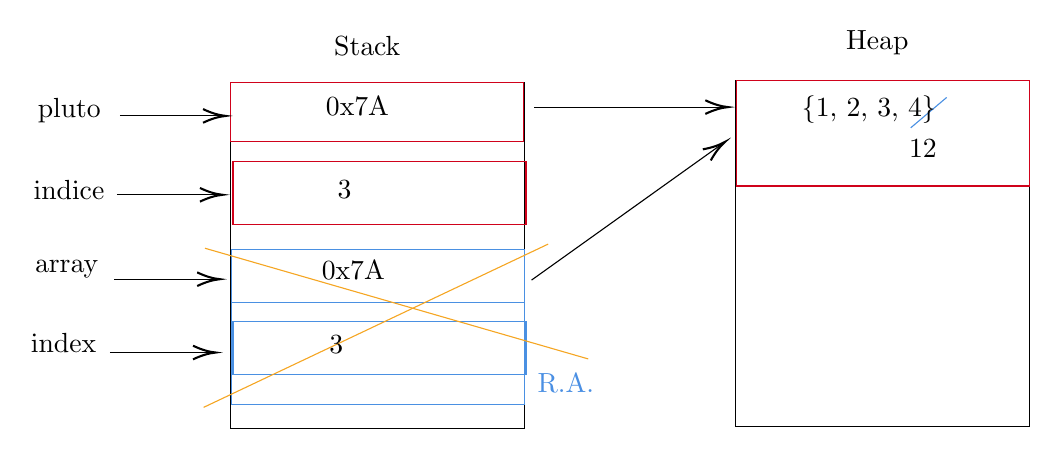
\begin{tikzpicture}[x=0.75pt,y=0.75pt,yscale=-1,xscale=1]
    %Shape: Rectangle [id:dp7152478227238795] 
    \draw   (174.67,70.33) -- (316.33,70.33) -- (316.33,237) -- (174.67,237) -- cycle ;
    %Shape: Rectangle [id:dp15757574158684595] 
    \draw   (418,69.67) -- (559.67,69.67) -- (559.67,236.33) -- (418,236.33) -- cycle ;
    %Shape: Rectangle [id:dp2724644334512444] 
    \draw  [color={rgb, 255:red, 208; green, 2; blue, 27 }  ,draw opacity=1 ] (174.67,70.33) -- (315.83,70.33) -- (315.83,99.08) -- (174.67,99.08) -- cycle ;
    %Straight Lines [id:da24565300060639061] 
    \draw    (121.33,86.58) -- (170.33,86.58) ;
    \draw [shift={(172.33,86.58)}, rotate = 180] [color={rgb, 255:red, 0; green, 0; blue, 0 }  ][line width=0.75]    (10.93,-3.29) .. controls (6.95,-1.4) and (3.31,-0.3) .. (0,0) .. controls (3.31,0.3) and (6.95,1.4) .. (10.93,3.29)   ;
    %Shape: Rectangle [id:dp552789858104063] 
    \draw  [color={rgb, 255:red, 208; green, 2; blue, 27 }  ,draw opacity=1 ] (175.83,108.33) -- (317,108.33) -- (317,139) -- (175.83,139) -- cycle ;
    %Straight Lines [id:da3542563643066503] 
    \draw    (119.83,124.58) -- (168.83,124.58) ;
    \draw [shift={(170.83,124.58)}, rotate = 180] [color={rgb, 255:red, 0; green, 0; blue, 0 }  ][line width=0.75]    (10.93,-3.29) .. controls (6.95,-1.4) and (3.31,-0.3) .. (0,0) .. controls (3.31,0.3) and (6.95,1.4) .. (10.93,3.29)   ;
    %Shape: Rectangle [id:dp635476864014964] 
    \draw  [color={rgb, 255:red, 208; green, 2; blue, 27 }  ,draw opacity=1 ] (418.5,69.67) -- (559.67,69.67) -- (559.67,120.33) -- (418.5,120.33) -- cycle ;
    %Straight Lines [id:da9897668665469099] 
    \draw    (321,82.33) -- (412.33,82.33) ;
    \draw [shift={(414.33,82.33)}, rotate = 180] [color={rgb, 255:red, 0; green, 0; blue, 0 }  ][line width=0.75]    (10.93,-3.29) .. controls (6.95,-1.4) and (3.31,-0.3) .. (0,0) .. controls (3.31,0.3) and (6.95,1.4) .. (10.93,3.29)   ;
    %Shape: Rectangle [id:dp5090426024134677] 
    \draw  [color={rgb, 255:red, 74; green, 144; blue, 226 }  ,draw opacity=1 ] (175.17,151) -- (316.33,151) -- (316.33,225.67) -- (175.17,225.67) -- cycle ;
    %Straight Lines [id:da513981228993915] 
    \draw    (118.5,165.25) -- (167.5,165.25) ;
    \draw [shift={(169.5,165.25)}, rotate = 180] [color={rgb, 255:red, 0; green, 0; blue, 0 }  ][line width=0.75]    (10.93,-3.29) .. controls (6.95,-1.4) and (3.31,-0.3) .. (0,0) .. controls (3.31,0.3) and (6.95,1.4) .. (10.93,3.29)   ;
    %Straight Lines [id:da8146722663255233] 
    \draw    (116.5,200.58) -- (165.5,200.58) ;
    \draw [shift={(167.5,200.58)}, rotate = 180] [color={rgb, 255:red, 0; green, 0; blue, 0 }  ][line width=0.75]    (10.93,-3.29) .. controls (6.95,-1.4) and (3.31,-0.3) .. (0,0) .. controls (3.31,0.3) and (6.95,1.4) .. (10.93,3.29)   ;
    %Shape: Rectangle [id:dp5414509911095386] 
    \draw  [color={rgb, 255:red, 74; green, 144; blue, 226 }  ,draw opacity=1 ] (175.17,151) -- (316.33,151) -- (316.33,176.33) -- (175.17,176.33) -- cycle ;
    %Shape: Rectangle [id:dp17471834612078319] 
    \draw  [color={rgb, 255:red, 74; green, 144; blue, 226 }  ,draw opacity=1 ] (175.83,185.67) -- (317,185.67) -- (317,211) -- (175.83,211) -- cycle ;
    %Straight Lines [id:da13256348158375997] 
    \draw    (319.67,165.67) -- (411.37,100.16) ;
    \draw [shift={(413,99)}, rotate = 144.46] [color={rgb, 255:red, 0; green, 0; blue, 0 }  ][line width=0.75]    (10.93,-3.29) .. controls (6.95,-1.4) and (3.31,-0.3) .. (0,0) .. controls (3.31,0.3) and (6.95,1.4) .. (10.93,3.29)   ;
    %Straight Lines [id:da18892227014269014] 
    \draw [color={rgb, 255:red, 74; green, 144; blue, 226 }  ,draw opacity=1 ]   (519.67,77.67) -- (502.33,92.33) ;
    %Straight Lines [id:da5546473880922558] 
    \draw [color={rgb, 255:red, 245; green, 166; blue, 35 }  ,draw opacity=1 ]   (327.67,148.33) -- (161.67,227) ;
    %Straight Lines [id:da23612180022025553] 
    \draw [color={rgb, 255:red, 245; green, 166; blue, 35 }  ,draw opacity=1 ]   (162.33,150.33) -- (347,203.67) ;
    
    % Text Node
    \draw (223.33,47) node [anchor=north west][inner sep=0.75pt]   [align=left] {Stack};
    % Text Node
    \draw (470,44.33) node [anchor=north west][inner sep=0.75pt]   [align=left] {Heap};
    % Text Node
    \draw (80.5,76.83) node [anchor=north west][inner sep=0.75pt]   [align=left] {pluto};
    % Text Node
    \draw (219.33,75.83) node [anchor=north west][inner sep=0.75pt]   [align=left] {0x7A};
    % Text Node
    \draw (225,116.5) node [anchor=north west][inner sep=0.75pt]   [align=left] {3};
    % Text Node
    \draw (448.67,75.83) node [anchor=north west][inner sep=0.75pt]   [align=left] {\{1, 2, 3, 4\}};
    % Text Node
    \draw (78.5,116.17) node [anchor=north west][inner sep=0.75pt]   [align=left] {indice};
    % Text Node
    \draw (79.17,154.83) node [anchor=north west][inner sep=0.75pt]   [align=left] {array};
    % Text Node
    \draw (77.17,190.17) node [anchor=north west][inner sep=0.75pt]   [align=left] {index};
    % Text Node
    \draw (217.33,155.17) node [anchor=north west][inner sep=0.75pt]   [align=left] {0x7A};
    % Text Node
    \draw (221,191.17) node [anchor=north west][inner sep=0.75pt]   [align=left] {3};
    % Text Node
    \draw (321.33,209.67) node [anchor=north west][inner sep=0.75pt]   [align=left] {\textcolor[rgb]{0.29,0.56,0.89}{R.A.}};
    % Text Node
    \draw (500.33,96.67) node [anchor=north west][inner sep=0.75pt]   [align=left] {12};    
\end{tikzpicture}

\textbf{Nota:} in questo caso il valore dell'array effettivamente cambia.


\vspace{1cm}
\subsubsection{Stringhe}
\begin{lstlisting}[style=java]
    String frase = "ciao";

    modificaStringa(frase);

    modificaStringa(frase) {
        frase += aggiunta;
    }
\end{lstlisting}
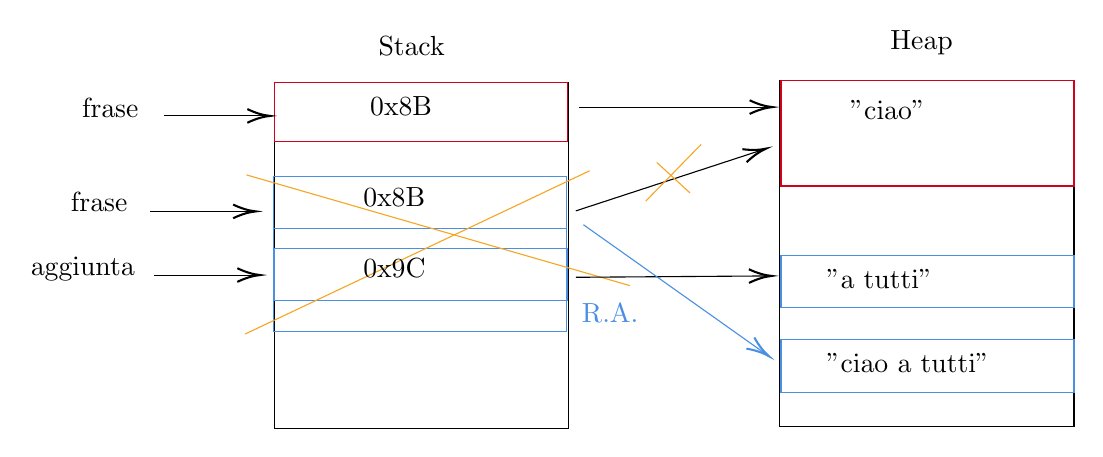
\begin{tikzpicture}[x=0.75pt,y=0.75pt,yscale=-1,xscale=1]
    %Shape: Rectangle [id:dp13936225442535932] 
    \draw   (169.67,64.33) -- (311.33,64.33) -- (311.33,231) -- (169.67,231) -- cycle ;
    %Shape: Rectangle [id:dp14499894212993758] 
    \draw   (413,63.67) -- (554.67,63.67) -- (554.67,230.33) -- (413,230.33) -- cycle ;
    %Shape: Rectangle [id:dp08018526916467927] 
    \draw  [color={rgb, 255:red, 208; green, 2; blue, 27 }  ,draw opacity=1 ] (169.67,64.33) -- (310.83,64.33) -- (310.83,93.08) -- (169.67,93.08) -- cycle ;
    %Straight Lines [id:da11760460213770985] 
    \draw    (116.33,80.58) -- (165.33,80.58) ;
    \draw [shift={(167.33,80.58)}, rotate = 180] [color={rgb, 255:red, 0; green, 0; blue, 0 }  ][line width=0.75]    (10.93,-3.29) .. controls (6.95,-1.4) and (3.31,-0.3) .. (0,0) .. controls (3.31,0.3) and (6.95,1.4) .. (10.93,3.29)   ;
    %Shape: Rectangle [id:dp43573129501262264] 
    \draw  [color={rgb, 255:red, 208; green, 2; blue, 27 }  ,draw opacity=1 ] (413.5,63.67) -- (554.67,63.67) -- (554.67,114.33) -- (413.5,114.33) -- cycle ;
    %Straight Lines [id:da41816903302987796] 
    \draw    (316,76.33) -- (407.33,76.33) ;
    \draw [shift={(409.33,76.33)}, rotate = 180] [color={rgb, 255:red, 0; green, 0; blue, 0 }  ][line width=0.75]    (10.93,-3.29) .. controls (6.95,-1.4) and (3.31,-0.3) .. (0,0) .. controls (3.31,0.3) and (6.95,1.4) .. (10.93,3.29)   ;
    %Shape: Rectangle [id:dp2394910475477957] 
    \draw  [color={rgb, 255:red, 74; green, 144; blue, 226 }  ,draw opacity=1 ] (168.83,109.67) -- (310,109.67) -- (310,184.33) -- (168.83,184.33) -- cycle ;
    %Straight Lines [id:da997394246028355] 
    \draw    (109.5,126.58) -- (158.5,126.58) ;
    \draw [shift={(160.5,126.58)}, rotate = 180] [color={rgb, 255:red, 0; green, 0; blue, 0 }  ][line width=0.75]    (10.93,-3.29) .. controls (6.95,-1.4) and (3.31,-0.3) .. (0,0) .. controls (3.31,0.3) and (6.95,1.4) .. (10.93,3.29)   ;
    %Shape: Rectangle [id:dp4374515201422946] 
    \draw  [color={rgb, 255:red, 74; green, 144; blue, 226 }  ,draw opacity=1 ] (168.83,109.67) -- (310,109.67) -- (310,135) -- (168.83,135) -- cycle ;
    %Shape: Rectangle [id:dp2163776799805549] 
    \draw  [color={rgb, 255:red, 74; green, 144; blue, 226 }  ,draw opacity=1 ] (169.5,144.33) -- (310.67,144.33) -- (310.67,169.67) -- (169.5,169.67) -- cycle ;
    %Straight Lines [id:da700896560452315] 
    \draw    (314.67,126.33) -- (404.43,96.96) ;
    \draw [shift={(406.33,96.33)}, rotate = 161.88] [color={rgb, 255:red, 0; green, 0; blue, 0 }  ][line width=0.75]    (10.93,-3.29) .. controls (6.95,-1.4) and (3.31,-0.3) .. (0,0) .. controls (3.31,0.3) and (6.95,1.4) .. (10.93,3.29)   ;
    %Straight Lines [id:da3667468395627571] 
    \draw [color={rgb, 255:red, 245; green, 166; blue, 35 }  ,draw opacity=1 ]   (321.33,107) -- (155.33,185.67) ;
    %Straight Lines [id:da8384101288758695] 
    \draw [color={rgb, 255:red, 245; green, 166; blue, 35 }  ,draw opacity=1 ]   (156,109) -- (340.67,162.33) ;
    %Straight Lines [id:da5288368243003695] 
    \draw    (111.5,157.25) -- (160.5,157.25) ;
    \draw [shift={(162.5,157.25)}, rotate = 180] [color={rgb, 255:red, 0; green, 0; blue, 0 }  ][line width=0.75]    (10.93,-3.29) .. controls (6.95,-1.4) and (3.31,-0.3) .. (0,0) .. controls (3.31,0.3) and (6.95,1.4) .. (10.93,3.29)   ;
    %Straight Lines [id:da5857553231554516] 
    \draw    (314.67,158.33) -- (407,157.68) ;
    \draw [shift={(409,157.67)}, rotate = 179.6] [color={rgb, 255:red, 0; green, 0; blue, 0 }  ][line width=0.75]    (10.93,-3.29) .. controls (6.95,-1.4) and (3.31,-0.3) .. (0,0) .. controls (3.31,0.3) and (6.95,1.4) .. (10.93,3.29)   ;
    %Shape: Rectangle [id:dp42851658404574666] 
    \draw  [color={rgb, 255:red, 74; green, 144; blue, 226 }  ,draw opacity=1 ] (413.5,147.67) -- (554.67,147.67) -- (554.67,173) -- (413.5,173) -- cycle ;
    %Straight Lines [id:da6289471960686158] 
    \draw [color={rgb, 255:red, 245; green, 166; blue, 35 }  ,draw opacity=1 ]   (375,94.33) -- (348.33,121.67) ;
    %Straight Lines [id:da5091858353952797] 
    \draw [color={rgb, 255:red, 245; green, 166; blue, 35 }  ,draw opacity=1 ]   (353.67,103) -- (369.67,117.67) ;
    %Straight Lines [id:da22966292357943108] 
    \draw [color={rgb, 255:red, 74; green, 144; blue, 226 }  ,draw opacity=1 ]   (318.33,133) -- (406.04,195.18) ;
    \draw [shift={(407.67,196.33)}, rotate = 215.33] [color={rgb, 255:red, 74; green, 144; blue, 226 }  ,draw opacity=1 ][line width=0.75]    (10.93,-3.29) .. controls (6.95,-1.4) and (3.31,-0.3) .. (0,0) .. controls (3.31,0.3) and (6.95,1.4) .. (10.93,3.29)   ;
    %Shape: Rectangle [id:dp15109834109667186] 
    \draw  [color={rgb, 255:red, 74; green, 144; blue, 226 }  ,draw opacity=1 ] (413.5,188.33) -- (554.67,188.33) -- (554.67,213.67) -- (413.5,213.67) -- cycle ;
    
    % Text Node
    \draw (218.33,41) node [anchor=north west][inner sep=0.75pt]   [align=left] {Stack};
    % Text Node
    \draw (465,38.33) node [anchor=north west][inner sep=0.75pt]   [align=left] {Heap};
    % Text Node
    \draw (75.5,70.83) node [anchor=north west][inner sep=0.75pt]   [align=left] {frase};
    % Text Node
    \draw (214.33,69.83) node [anchor=north west][inner sep=0.75pt]   [align=left] {0x8B};
    % Text Node
    \draw (445.67,71.83) node [anchor=north west][inner sep=0.75pt]   [align=left] {"ciao"};
    % Text Node
    \draw (70.17,116.17) node [anchor=north west][inner sep=0.75pt]   [align=left] {frase};
    % Text Node
    \draw (211,113.83) node [anchor=north west][inner sep=0.75pt]   [align=left] {0x8B};
    % Text Node
    \draw (316.33,169.67) node [anchor=north west][inner sep=0.75pt]   [align=left] {\textcolor[rgb]{0.29,0.56,0.89}{R.A.}};
    % Text Node
    \draw (50.83,147.5) node [anchor=north west][inner sep=0.75pt]   [align=left] {aggiunta};
    % Text Node
    \draw (211,147.83) node [anchor=north west][inner sep=0.75pt]   [align=left] {0x9C};
    % Text Node
    \draw (434.33,153.17) node [anchor=north west][inner sep=0.75pt]   [align=left] {"a tutti"};
    % Text Node
    \draw (434.33,193.83) node [anchor=north west][inner sep=0.75pt]   [align=left] {"ciao a tutti"};    
\end{tikzpicture}    

\textbf{Nota:} in questo caso il valore della stringa non cambia.



\end{document}